
\chapter{ಕಾಲೇಜಿನ ದಿನಗಳು}

ನರೇಂದ್ರ ಎನ್‍ಟ್ರೆನ್ಸ್ ಪರೀಕ್ಷೆಯಲ್ಲಿ ಪಾಸುಮಾಡಿದಮೇಲೆ ೧೮೭೯ರಲ್ಲಿ ಪ್ರೆಸಿಡೆನ್ಸಿ\break ಕಾಲೇಜಿಗೆ ಸೇರಿದ. ಕೆಲವು ಕಾಲದ ಮೇಲೆ ಅದನ್ನು ಬಿಟ್ಟು ಸ್ಕಾಟಿಶ್ ಚರ್ಚ್ ಕಾಲೇಜಿಗೆ ಸೇರಿದ. ಎನ್‍ಟ್ರೆನ್ಸ್ ಪರೀಕ್ಷೆಗೆ ಮೂರು ವರ್ಷಗಳ ಪಾಠವನ್ನು ಓದಬೇಕಾಗಿದ್ದುದರಿಂದ ಮನಸ್ಸಿಗೆ ತೀವ್ರ ತೊಂದರೆಯಾಗಿ ನರಗಳ ದೌರ್ಬಲ್ಯದಿಂದ ನರಳಿ ದೇಹಾರೋಗ್ಯ ಕೆಟ್ಟಿತು. ಹವಾ ಬದಲಾವಣೆಗಾಗಿ ವಿಶ್ವನಾಥದತ್ತ ನರೇಂದ್ರನನ್ನು ಕೆಲವು ತಿಂಗಳು ಗಯಾಗೆ ತನ್ನ ನೆಂಟರೊಬ್ಬರ ಮನೆಗೆ ಕಳುಹಿಸಿದ. ಆರೋಗ್ಯ ಉತ್ತಮಗೊಂಡಮೇಲೆ ವರುಷದ ಪರೀಕ್ಷೆಗೆ ಮುಂಚೆ ಕಲ್ಕತ್ತೆಗೆ ಪುನಃ ನರೇಂದ್ರ ಬಂದ. ಬಂದವನೆ ಪರೀಕ್ಷೆಗೆ ಸಂಬಂಧಪಟ್ಟ ಪುಸ್ತಕಗಳನ್ನೆಲ್ಲ ಓದಿ ಪರೀಕ್ಷೆಯಲ್ಲಿ ಎರಡನೇ ದರ್ಜೆಯಲ್ಲಿ ಉತ್ತೀರ್ಣನಾದನು.

ಕಾಲೇಜಿಗೆ ಸೇರಿದ ಮೇಲೆ ಹಿಂದಿನ ಲಘುವಾದ ಆಟಗಳು, ಹಾಸ್ಯ ಪರಿಹಾಸ್ಯಗಳು ಎಲ್ಲವನ್ನೂ ಬಿಟ್ಟು ವಿಷಯಸಂಗ್ರಹದ ಕಡೆ ಗಮನವಿಟ್ಟನು. ನರೇಂದ್ರನ ರುಚಿ ಬಹುಮುಖವಾದುದು. ಸಾಹಿತ್ಯ, ಖಗೋಳಶಾಸ್ತ್ರ, ಇತಿಹಾಸ, ಸಮಾಜ ವಿಜ್ಞಾನ, ತತ್ತ್ವಶಾಸ್ತ್ರ, ತರ್ಕ ಮುಂತಾದವುಗಳ ಮೇಲಿನ ಪುಸ್ತಕಗಳನ್ನೆಲ್ಲ ಓದುತ್ತಿದ್ದ. ಅವುಗಳನ್ನು ಕುರಿತು ಆಯಾ ವಿಷಯಗಳಲ್ಲಿ ನುರಿತ ಉಪಾಧ್ಯಾಯರೊಡನೆ ಮಾತನಾಡುತ್ತಿದ್ದ. ಅನೇಕ ಉಪಾಧ್ಯಾಯರಿಗೆ ಅವನನ್ನು ಕಂಡರೆ ಬಹಳ ಪ್ರೀತಿ. ಆ ಕಾಲೇಜಿನ ಪ್ರಿನ್ಸಿಪಾಲರಾದ ವಿಲಿಯಂ ಹೇಸ್ಟಿ ಎನ್ನುವವರೇ ಹೀಗೆ ಬರೆಯುತ್ತಾರೆ: “ನರೇಂದ್ರನದು ನಿಜವಾಗಿಯೂ ಅದ್ಭುತ ಪ್ರತಿಭೆ. ನಾನು ಪ್ರಪಂಚದಲ್ಲಿ ಬೇಕಾದಷ್ಟು ಸಂಚಾರ ಮಾಡಿರುವೆನು. ಜರ್ಮನ್ ವಿಶ್ವವಿದ್ಯಾನಿಲಯಗಳಲ್ಲಿ ತತ್ತ್ವಶಾಸ್ತ್ರ ಅಧ್ಯಯನ ಮಾಡುವ ವಿದ್ಯಾರ್ಥಿವರ್ಗದಲ್ಲಿ ಕೂಡ ಇಷ್ಟೊಂದು ಬುದ್ಧಿವಂತನಾದ ಹುಡುಗನನ್ನು ನಾನು ಕಂಡಿಲ್ಲ. ನರೇಂದ್ರ ಜೀವನದಲ್ಲಿ ಖ್ಯಾತಿಯನ್ನು ಗಳಿಸುವುದರಲ್ಲಿ ಸಂದೇಹವಿಲ್ಲ.”

ನರೇಂದ್ರನ ವಾಚಾಳಿತನ ಅವನು ಕಾಲೇಜಿನಲ್ಲಿ ಓದುತ್ತಿದ್ದ ಕಾಲದಲ್ಲಿಯೇ ನಮಗೆ ವೇದ್ಯವಾಗುವುದು. ಒಂದು ಸಲ ಬಹಳ ವರ್ಷಗಳು ಕೆಲಸ ಮಾಡಿದ ಪ್ರಾಧ್ಯಾಪಕರೊಬ್ಬರು ನಿವೃತ್ತರಾಗುವ ಸಮಯ ಬಂದಿತು. ವಿದ್ಯಾರ್ಥಿಗಳೆಲ್ಲ ಸೇರಿ ಅವರನ್ನು ಬೀಳ್ಕೊಡುವುದಕ್ಕೆ ಒಂದು ಸಮಾರಂಭವನ್ನು ಯೋಜಿಸಿದರು. ಅದಕ್ಕೆ ಕಲ್ಕತ್ತೆಯ ಪ್ರಖ್ಯಾತ ವಾಗ್ಮಿಗಳಾದ ಸುರೇಂದ್ರನಾಥ ಬ್ಯಾನರ್ಜಿ ಅವರನ್ನು ಅಧ್ಯಕ್ಷರನ್ನಾಗಿ ಮಾಡಿದರು. ಆಗ ವಿದ್ಯಾರ್ಥಿಗಳ ಪರವಾಗಿ ಒಬ್ಬರು ಮಾತನಾಡಬೇಕಾಗಿ ಬಂದಿತು. ಸುರೇಂದ್ರನಾಥ ಬ್ಯಾನರ್ಜಿಯಂತಹ ವಾಗ್ಮಿಗಳ ಎದುರಿಗೆ ಅನೇಕ ನುರಿತ ವಾಚಾಳಿಗಳೇ ಅಂಜುವರು ತಮ್ಮ ಬಾಯನ್ನು ತೆರೆಯುವುದಕ್ಕೆ. ಎಲ್ಲರೂ ನರೇಂದ್ರನೆ ಆ ಭಾಷಣವನ್ನು ಮಾಡಬೇಕೆಂದು ಕೇಳಿಕೊಂಡರು. ನರೇಂದ್ರ ಅದನ್ನು ಯಶಸ್ವಿಯಾಗಿ ನೆರವೇರಿಸಿದ. ನಿವೃತ್ತರಾಗುವ ಪ್ರಾಧ್ಯಾಪಕರ ಗುಣಗಳನ್ನು ಹೃದಯಂಗಮವಾಗಿ ಚಿತ್ರಿಸಿ ಅವರಿಗೆ ವಿದ್ಯಾರ್ಥಿಗಳ ಪರವಾಗಿ ಅಭಿನಂದನೆಗಳನ್ನು ಅರ್ಪಿಸಿದ. ಆ ಭಾಷಣ ಬಹಳ ಚೆನ್ನಾಗಿತ್ತು. ಅಧ್ಯಕ್ಷರಾಗಿ ಬಂದಿದ್ದ ವಂಗದೇಶದ ಪ್ರಖ್ಯಾತ ವಾಗ್ಮಿ ಕೂಡ ಮುಗ್ಧರಾಗಿ ಹೋದರು. ಅವರು ನರೇಂದ್ರನ ಭಾಷಣವನ್ನು ಶ್ಲಾಘಿಸಿದರು.

ನರೇಂದ್ರನ ಮಾತು ಕಥೆಗಳಲ್ಲಿ ಒಂದು ಆಕರ್ಷಣೆ ಇತ್ತು. ಅವನ ಮಾತು ಕಿವಿಗೆ\break ಇಂಪಾಗಿತ್ತು.ಅದೊಂದು ಸಂಗೀತದಂತೆ ಇತ್ತು ಎಂದು ಕೇಳಿದವರು ಹೇಳುವರು. ಅದರಲ್ಲಿರುವ ವಿಚಾರಸರಣಿ ಕೇಳುವವರ ಕಿವಿಗೊಂದು ಹಬ್ಬ. ಅದನ್ನು ಕೇಳಬೇಕೆಂದೇ ಅವನ ಕೆಲವು ವಿದ್ಯಾರ್ಥಿ ಸ್ನೇಹಿತರು ಯಾವುದಾದರೂ ಪ್ರಶ್ನೆಯನ್ನು ಹಾಕುತ್ತಿದ್ದರು. ನರೇಂದ್ರ ಅದನ್ನು ವಿವರಿಸುವಾಗ ಮತ್ತೆಲ್ಲಿಯೂ ಕಾಣದ ಸ್ವತಂತ್ರ ವಿಚಾರಸರಣಿ ಅದರಲ್ಲಿರುತ್ತಿತ್ತು.

ವಿಶ್ವನಾಥದತ್ತ ಮಗನ ಬುದ್ಧಿಶಕ್ತಿಯನ್ನು ಪ್ರಚೋದಿಸಲು ಹೇಗೆ ಅವಕಾಶವನ್ನು ಕಲ್ಪಿಸುತ್ತಿದ್ದನೋ ಹಾಗೆಯೇ ಅವನ ಕಲಾಭಿರುಚಿಗೂ ಪ್ರೋತ್ಸಾಹವನ್ನು ನೀಡಿದನು. ಮೊದಲಿನಿಂದಲೂ ನರೇಂದ್ರನಿಗೆ ಬಹಳ ಮಧುರವಾದ ಕಂಠವಿದ್ದುದು ತಂದೆಗೆ ಗೊತ್ತಿತ್ತು. ಅವನು ಹಾಡುಗಳನ್ನು ಚೆನ್ನಾಗಿ ಹಾಡುತ್ತಿದ್ದ. ಅದನ್ನು ಶಾಸ್ತ್ರೀಯ ರೀತಿ ಚೆನ್ನಾಗಿ ಅಭ್ಯಾಸ ಮಾಡಿಕೊಳ್ಳಲಿ ಎಂದು ಇಬ್ಬರು ಸಂಗೀತ ಉಪಾಧ್ಯಾಯರುಗಳನ್ನು ನೇಮಕ ಮಾಡಿದ. ಒಬ್ಬ ಹಿಂದೂಸ್ಥಾನಿ ಸಂಗೀತವನ್ನು ಕಲಿಸುವುದಕ್ಕೆ. ಅವನ ಹೆಸರೇ ಉಸ್ತಾದ್ ಅಹಮದ್ ಖಾನ್. ಬಂಗಾಳಿಯ ಭಕ್ತಿಗೀತೆಗಳನ್ನು ಕಲಿಸುವುದಕ್ಕೆ ಬೇಣೀಪಾಲ್ ಎಂಬ ಮತ್ತೊಬ್ಬನನ್ನು ನೇಮಕಮಾಡಿದ. ನರೇಂದ್ರ ಶಾಸ್ತ್ರೀಯವಾಗಿ ಹಾಡುವುದರಲ್ಲಿ ಪಾರಂಗತನಾದನು. ಜೊತೆಗೆ ಹಲವು ವಾದ್ಯಗಳನ್ನು ಬಾರಿಸುವುದರಲ್ಲಿಯೂ ಅಗ್ರಗಣ್ಯನಾದನು. ನಾವು ಮೊದಲೇ ಹೇಳಿದೆವು ಆಟ ಪಾಠ ಒಂದು ಜೀವಿಯಲ್ಲಿ ಒಂದೇ ಪ್ರಮಾಣದಲ್ಲಿರುವುದು ಅಪರೂಪ ಎಂದು. ಅದರಂತೆಯೇ ಅಷ್ಟೇ ಅಪರೂಪ, ಓದುವುದರಲ್ಲಿ ಮುಂದಾಗಿದ್ದು, ಸಂಗೀತದಲ್ಲಿಯೂ ಅಷ್ಟೇ ಅಭಿರುಚಿಯಿರುವುದು. ಅನೇಕ ವೇಳೆ ಸಂಗೀತಶಾಸ್ತ್ರದಲ್ಲಿ ಮುಂದುವರಿದವರು ವಿದ್ಯಾಭ್ಯಾಸದ ಕೆಳಮಟ್ಟದಲ್ಲಿಯೇ ಸೋತುಹೋಗುವರು. ಆದರೆ ನರೇಂದ್ರನಾಥನದಾದರೊ ಅದ್ಭುತ ವ್ಯಕ್ತಿತ್ವ. ಪ್ರಕೃತಿ ಅಘಟಿತ ಘಟನೆಗಳನ್ನೆಲ್ಲ ಇಲ್ಲಿ ಒಂದುಗೂಡಿಸಿ ಇರುವುದನ್ನು ನೋಡುವೆವು. ಒಂದು ಸಲ ಶಾಲೆಯ ಪ್ರಾಧ್ಯಾಪಕರು ಬರುವುದು ತಡವಾಯಿತು. ಹುಡುಗರು ನರೇಂದ್ರನನ್ನು ಒಂದು ಹಾಡನ್ನು ಹೇಳುವಂತೆ ಕೇಳಿಕೊಂಡರು. ನರೇಂದ್ರನು ತನ್ನ ಕಿನ್ನರ ಕಂಠದಲ್ಲಿ ಹಾಡುತ್ತಿದ್ದಾಗ ಮಧ್ಯದಲ್ಲಿ ಪ್ರಾಧ್ಯಾಪಕರು ಬಂದರು. ಅವರು ಕ್ಲಾಸಿನ ರೂಮಿನ ಹೊರಗಡೆಯೆ ನಿಂತುಕೊಂಡು ಅದು ಪೂರ್ಣವಾಗುವವರೆಗೂ ಕೇಳಿ, ಅನಂತರ ಅದು ಮುಗಿದಮೇಲೆ ಒಳಗೆ ಪ್ರವೇಶಿಸಿದರು. ಹಾಡುತ್ತಿದ್ದವನನ್ನು ಶ್ಲಾಘಿಸಿದರು. ನರೇಂದ್ರ ತಾನು ವಿದ್ಯಾರ್ಥಿದೆಸೆಯಲ್ಲಿರುವಾಗಲೇ ತನ್ನ ಸ್ನೇಹಿತನೊಬ್ಬನು ಸಂಗ್ರಹಿಸಿದ ಬಂಗಾಳಿ ಹಾಡುಗಳಿಗೆ ಒಂದು ಪಾಂಡಿತ್ಯಪೂರಿತ ಮುನ್ನುಡಿಯನ್ನು ಬರೆದುಕೊಟ್ಟನು. ಮುಂದೆ ಇವನ ಗುರುಗಳಾದ ಶ‍್ರೀರಾಮಕೃಷ್ಣರನ್ನು ಪ್ರಥಮ ಬಾರಿ ಆಕರ್ಷಿಸಿದ್ದೂ ಕೂಡ ನರೇಂದ್ರನ ಹಾಡೇ. ೧೮೮೧ರಲ್ಲಿ ಶ‍್ರೀರಾಮಕೃಷ್ಣರು ಕಲ್ಕತ್ತೆಯಲ್ಲಿ ಸುರೇಂದ್ರನಾಥಮಿತ್ರನೆಂಬ ಗೃಹಸ್ಥಭಕ್ತನ ಮನೆಗೆ ಬಂದಿದ್ದರು. ಅಲ್ಲಿ ಹಾಡುವವರು ಯಾರೂ ಅಂದು ಸಿಕ್ಕಿರಲಿಲ್ಲ. ನರೇಂದ್ರನಿಗೆ ಪರಿಚಯವಿದ್ದವರೊಬ್ಬರು ಅವನನ್ನು ಮನೆಯಿಂದ ಕರೆಸಿ ನರೇಂದ್ರನಿಂದ ಹಾಡನ್ನು ಹಾಡಿಸಿದರು. ಶ‍್ರೀರಾಮಕೃಷ್ಣರು ನರೇಂದ್ರನ ಹಾಡಿನ ಕೆಲವು ಪಲ್ಲವಿಗಳನ್ನು ಕೇಳುವುದೇ ತಡ ಸಮಾಧಿಮಗ್ನರಾದರು. ಪ್ರಕೃತಿಸ್ಥರಾದಮೇಲೆ ನರೇಂದ್ರನ ಕಡೆ ನೋಡಿದರು. ಕಲ್ಕತ್ತೆಯ ಮಧ್ಯದಲ್ಲಿ ಇಂತಹ ಹುಡುಗ ಇರಬಲ್ಲನೆ ಎಂದು ಆಶ್ಚರ್ಯಪಟ್ಟರು. ಅವನಿಗೆ ಒಮ್ಮೆ ದಕ್ಷಿಣೇಶ್ವರಕ್ಕೆ ಬಾ ಎಂದು ಆಮಂತ್ರಣವನ್ನು ಕೊಟ್ಟಿದ್ದರು. ಆದರೆ ಇಬ್ಬರಿಗೂ ಯಾವ ಪರಿಚಯವೂ ಇರಲಿಲ್ಲ. ಅದು ಇಲ್ಲಿಗೇ ಪರ‍್ಯವಸಾನವಾಗಿತ್ತು.

ನರೇಂದ್ರ ಕಾಲೇಜಿನಲ್ಲಿ ಓದುತ್ತಿದ್ದಾಗ ಹಿಂದೊಮ್ಮೆ ಶ‍್ರೀರಾಮಕೃಷ್ಣರ ವಿಷಯವನ್ನು ತನ್ನ ಪ್ರಿನ್ಸಿಪಾಲರಾದ ವಿಲಿಯಂ ಹೇಸ್ಟಿಯವರ ಬಾಯಿಂದ ಕೇಳಿದ್ದ. ಒಂದು ದಿನ ಇಂಗ್ಲೀಷ್ ಪ್ರೊಫೆಸರ್ ನರೇಂದ್ರನ ಕ್ಲಾಸಿಗೆ ಬರಲಿಲ್ಲ. ಅಂದು ಪ್ರಿನ್ಸಿಪಾಲ್ ಹೇಸ್ಟಿ ಅವರು ವರ್ಡ್ಸವರ್ತ್ ಕವಿಯ \enginline{Excursion} ಎಂಬ ಕವನವನ್ನು ಕುರಿತು ಪಾಠ ಹೇಳುತ್ತಿದ್ದರು. ಅದರಲ್ಲಿ ಕವಿ ಪ್ರಕೃತಿಯ ಸೌಂದರ‍್ಯವನ್ನು ನೋಡುತ್ತ ನೋಡುತ್ತ ಕಾಲದೇಶದ ಪರಿವೆಯೆ ಇಲ್ಲದ ಒಂದು ಸಮಾಧಿ ಸ್ಥಿತಿಯನ್ನು ವಿವರಿಸುತ್ತಾನೆ. ಅದನ್ನು ಪ್ರಿನ್ಸಿಪಾಲ್ ಹೇಸ್ಟಿ ವಿವರಿಸುವಾಗ ಹೇಳುತ್ತಾರೆ; “ಇಂತಹ ಅನುಭವ, ಶುದ್ಧವಾದ ಮನಸ್ಸು ಯಾವುದಾದರೂ ಒಂದು ವಸ್ತುವಿನ ಮೇಲೆ ಏಕಾಗ್ರವಾದಾಗ ಬರುವುದು. ಇಂದಿನ ಕಾಲದಲ್ಲಿ ಇಂತಹ ಅನುಭವಗಳು ವ್ಯಕ್ತಿಗೆ ಆಗುವುದು ಅಪರೂಪ. ನಾನು ಅಂತಹ ಧ್ಯಾನಾವಸ್ಥೆಯನ್ನು ಪಡೆದ ಒಬ್ಬನನ್ನು ಮಾತ್ರ ನೋಡಿರುವೆನು. ಅವರೇ ದಕ್ಷಿಣೇಶ್ವರದಲ್ಲಿರುವ ಶ‍್ರೀರಾಮಕೃಷ್ಣ ಪರಮಹಂಸರು. ನೀವೇ ಅಲ್ಲಿಗೆ ಹೋಗಿ ನೋಡಿದರೆ ನಿಮಗೆ ಇದು ವೇದ್ಯವಾಗುವುದು.” ನರೇಂದ್ರ ಪ್ರಥಮ ಬಾರಿ ಶ‍್ರೀರಾಮಕೃಷ್ಣರ ಹೆಸರನ್ನು ಕೇಳಿದ್ದು ತನ್ನ ಪ್ರಿನ್ಸಿಪಾಲರಿಂದ.

ನರೇಂದ್ರನಿಗೆ ಯಾವಾಗಲೂ ಕಷ್ಟದಲ್ಲಿ ಬಿದ್ದಿದ್ದ ತನ್ನ ಸ್ನೇಹಿತರ ಮೇಲೆ ಅನುಕಂಪವಿತ್ತು. ಅವರ ಸಹಾಯಕ್ಕೆ ಇವನು ಎಷ್ಟು ಕಷ್ಟವನ್ನಾದರೂ ತೆಗೆದುಕೊಳ್ಳುತ್ತಿದ್ದನು. ಒಂದು ಸಲ ಪರೀಕ್ಷಾ ಸಮಯ ಸನ್ನಿಹಿತವಾಯಿತು. ಇವನ ಒಬ್ಬ ಸ್ನೇಹಿತ ವಿದ್ಯಾರ್ಥಿ ಫೀಜನ್ನು ಕಟ್ಟಿರಲಿಲ್ಲ. ಫೀಜನ್ನು ಕೊಡದೆ ಪರೀಕ್ಷೆಗೆ ಕುಳಿತುಕೊಳ್ಳುವಂತೆ ಇರಲಿಲ್ಲ. ಕಾಲೇಜಿನ ಸೂಪರಿಂಟೆಂಡೆಂಟರಿಗೆ ಆ ಹುಡುಗನ ಬಡತನವನ್ನು ವಿವರಿಸಿ ಅವನ ಕೈಯಿಂದ ಫೀಜು ಕೊಡಲು ಸಾಧ್ಯವಿಲ್ಲವೆಂದೂ ಅವನು ಹಾಗೆಯೇ ಪರೀಕ್ಷೆಗೆ ಕುಳಿತುಕೊಳ್ಳಲು ಅವಕಾಶ ಕೊಡಬೇಕೆಂದೂ ಕೇಳಿಕೊಂಡನು. ಆದರೆ ಮೊದಲು ಅದಕ್ಕೆ ಆತ ಒಪ್ಪಲಿಲ್ಲ. ಆತ ಪ್ರತಿದಿನವೂ ಗಾಳಿಯ ಸಂಚಾರಕ್ಕೆ ಒಂದು ದಿಕ್ಕಿಗೆ ಹೋಗುತ್ತಿದ್ದನು. ನರೇಂದ್ರನು ಆ ದಾರಿಯಲ್ಲಿ ಆತನಿಗೆ ಕಾಯುತ್ತಿದ್ದು, ಅವನು ಬಂದಮೇಲೆ ಹುಡುಗನ ಸ್ಥಿತಿಯನ್ನು ಪುನಃ ವಿವರಿಸಿ ಅವನಿಗೆ ಸಹಾಯ ಮಾಡಬೇಕೆಂದು ಕೋರಿಕೊಂಡನು. ಈ ಸಲ ಆತ ಫೀಜನ್ನು ಮಾಫಿ ಮಾಡಲು ಒಪ್ಪಿಕೊಂಡು ಆ ವಿದ್ಯಾರ್ಥಿಗೆ ಪರೀಕ್ಷೆಗೆ ಕೂಡಲು ಅವಕಾಶವನ್ನು ಕೊಟ್ಟನು.

ಬಂಗಾಳದೇಶದಲ್ಲಿ ಆಗ ಎದ್ದ ಒಂದು ಸಮಾಜ ಸುಧಾರಣೆಯ ಚಳುವಳಿ ಎಲ್ಲರನ್ನೂ ಆಕರ್ಷಿಸಿತು. ಅದೇ ಬ್ರಹ್ಮಸಮಾಜ. ರಾಜಾರಾಮ ಮೋಹನರಾಯನಿಂದ ಇದು ಸ್ಥಾಪಿತವಾಯಿತು. ಅಲ್ಲಿ ಉಪನಿಷತ್ತಿನ ಶುದ್ಧತತ್ತ್ವ ರೀತಿಯಲ್ಲಿ ದೇವರನ್ನು ಉಪಾಸನೆ ಮಾಡುವುದನ್ನು ಜಾರಿಗೆ ತಂದರು. ಇದು ಮಹಮ್ಮದೀಯ ಮತ್ತು ಕ್ರೈಸ್ತಧರ್ಮಗಳಿಗೂ ಹಿಂದೂಧರ್ಮಕ್ಕೂ ಆದ ಕ್ರಿಯೆ-ಪ್ರತಿಕ್ರಿಯೆಯಿಂದ ಹುಟ್ಟಿತು. ಹೊರಗಿನಿಂದ ಬಂದ ಧರ್ಮದವರು ಹಿಂದೂಗಳನ್ನು ವಿಗ್ರಹಾರಾಧಕರು ಎಂದು ಹಳಿಯುತ್ತಿದ್ದರು. ಆದರೆ ಹಿಂದೂ ಧರ್ಮದಲ್ಲಿ ವಿಗ್ರಹಾರಾಧನೆ ಕೇವಲ ಪ್ರಥಮ ಮೆಟ್ಟಲು. ಅದನ್ನೂ ಮೀರಿದವರಿಗೆ ಒಂದು ಸ್ಥಳವಿದೆ. ಬ್ರಹ್ಮನನ್ನು ಜೀವಿ ಹೇಗೆ ಬೇಕಾದರೂ ಉಪಾಸನೆ ಮಾಡಬಹುದು. ಆದರೆ ಅಂದಿನ ಕಾಲದಲ್ಲಿ ಮಹಮ್ಮದೀಯರು ಮತ್ತು ಕ್ರೈಸ್ತರಿಂದ ತಾವು ವಿಗ್ರಹಾರಾಧಕರ ಗುಂಪಿಗೆ ಸೇರಿದವರು ಎಂದು ಕರೆಸಿಕೊಳ್ಳುತ್ತಿದ್ದವರು ಹೇಗಾದರೂ ಆ ಟೀಕೆಯಿಂದ ಪಾರಾಗಬೇಕೆಂದು ಒಂದು ಪಂಥವನ್ನು ಸ್ಥಾಪಿಸಿ ಅಲ್ಲಿ ದೇವರನ್ನು ಕೇವಲ ಗುಣಗಳ ಮೂಲಕ ನಿರಾಕಾರವಾಗಿ\break ಆರಾಧಿಸಲು ಪ್ರಾರಂಭಿಸಿದರು. ಇದಕ್ಕೆ ಉಪನಿಷತ್ತಿನಿಂದ ಆಶ್ರಯವನ್ನು ಪಡೆದುಕೊಂಡರು. ಇದಕ್ಕೆ ಸೇರಿದವರು ವಿಗ್ರಹಗಳನ್ನು ಪೂಜಿಸುವುದಿಲ್ಲ. ದೇವರ ಅವತಾರಗಳನ್ನು ನಂಬುವುದಿಲ್ಲ. ಅವರಿಗೆ ಮಾನವ ಗುರುಗಳು ಬೇಕಾಗಿಲ್ಲ. ರಾಜಾರಾಮ ಮೋಹನನ ತರುವಾಯ ಇದಕ್ಕೆ ಮಹರ್ಷಿ ದೇವೇಂದ್ರನಾಥ ಠಾಕೂರ್ ಮತ್ತು ಕೇಶವಚಂದ್ರಸೇನರು ನಾಯಕರಾದರು. ಕೇಶವಚಂದ್ರಸೇನ ಇಂಗ್ಲೀಷ್ ಮತ್ತು ಬಂಗಾಳಿಯಲ್ಲಿ ಬಹಳ ಚೆನ್ನಾಗಿ ಮಾತನಾಡಬಲ್ಲವನಾಗಿದ್ದ. ಅನೇಕ ಜನ ಯುವಕರು ಅವನ ಉಪನ್ಯಾಸವನ್ನು ಕೇಳುವುದಕ್ಕೆ ಹೋಗುತ್ತಿದ್ದರು. ನರೇಂದ್ರನೂ ಕೂಡ ಕೇಶವಚಂದ್ರನ ಕೆಲವು ಉಪನ್ಯಾಸಗಳನ್ನು ಕೇಳಿದ. ಕೇಶವ ಕ್ರಮೇಣ ಆಧ್ಯಾತ್ಮಿಕಕ್ಕಿಂತ ಹೆಚ್ಚಾಗಿ ಸಮಾಜ ಸುಧಾರಣೆಯ ಕಡೆಗೆ ಗಮನವನ್ನು ಕೊಡಲು ಪ್ರಾರಂಭಿಸಿದನು. ಅದರಲ್ಲಿ ಜಾತಿಮತಗಳನ್ನು ಒಪ್ಪಿಕೊಳ್ಳದಿರುವುದು, ಸ್ತ್ರೀಯರಿಗೆ ವಿದ್ಯಾಭ್ಯಾಸವನ್ನು ಕೊಡುವುದು, ಅವರಿಗೆ ಪ್ರಾಪ್ತವಯಸ್ಸಾದ ಮೇಲೆಯೇ ಮದುವೆ ಮಾಡುವುದು ಇವುಗಳನ್ನೆಲ್ಲ ಜಾರಿಗೆ ತಂದರು. ಇವುಗಳೆಲ್ಲ ಯುವಕರಿಗೆ ತಾತ್ಕಾಲಿಕ ತೃಪ್ತಿಯನ್ನು ಕೊಟ್ಟವು. ಸಮಾಜ ಸುಧಾರಣೆಗಳು, ಜೀವಿಯ ಆಧ್ಯಾತ್ಮಿಕ ತೃಷೆಯನ್ನು ಹಿಂಗಿಸಲಾರವು. ಹುಡುಗಿಯರಿಗೆ ಪ್ರಾಪ್ತವಯಸ್ಸಾದ ಮೇಲೆಯೇ ಮದುವೆ ಮಾಡಬೇಕೆಂದು ಶಾಸನವನ್ನು ತಂದ ಕೇಶವಸೇನನೇ ತನ್ನ ಮಗಳಿಗೆ ಶ‍್ರೀಮಂತ ಮನೆತನದಿಂದ ವರನೊಬ್ಬ ಸಿಕ್ಕಿದಾಗ ಅವಳಿಗೆ ಅಷ್ಟು ವಯಸ್ಸಾಗಿಲ್ಲದೇ ಇದ್ದರೂ ಮಗಳನ್ನು ಮದುವೆ ಮಾಡಿಕೊಟ್ಟನು. ಇದು ಬ್ರಹ್ಮಸಮಾಜದಲ್ಲಿ ದೊಡ್ಡ ಆಂದೋಳನಕ್ಕೆ ಕಾರಣವಾಯಿತು. ಬ್ರಹ್ಮಸಮಾಜ ಎರಡು ಕವಲಾಗಿ ಒಡೆಯಿತು. ಕೇಶವಸೇನನು ಒಂದು ಪಂಗಡಕ್ಕೆ ಸೇರಿದನು. ಅವನಿಗೆ ವಿರೋಧವಾಗಿ ಪಂಡಿತ ಶಿವನಾಥ ಶಾಸ್ತ್ರಿ ಮತ್ತು ವಿಜಯಕೃಷ್ಣ ಗೋಸ್ವಾಮಿಗಳು ಮತ್ತೊಂದು ಶಾಖೆಗೆ ಸೇರಿದರು. ನರೇಂದ್ರ ಈ ಶಾಖೆಯ ಸದಸ್ಯನಾಗಿ ಅವರ ಪ್ರಾರ್ಥನೆ ಭಜನೆ ಮುಂತಾದುವುಗಳಲ್ಲಿ ಭಾಗವಹಿಸುತ್ತಿದ್ದ. ಅವು ತಾತ್ಕಾಲಿಕವಾಗಿ ಅವನಿಗೆ ಸ್ವಲ್ಪ ತೃಪ್ತಿಯನ್ನು ಕೊಟ್ಟಿದ್ದರೂ ಬಹಳ ದೂರದವರೆಗೆ ಅವನನ್ನು ಕರೆದುಕೊಂಡು ಹೋಗಲಿಲ್ಲ. ಅಲ್ಲಿ ದೇವರೊಂದಿಗೆ ಪ್ರತ್ಯಕ್ಷ ಸಂಬಂಧವನ್ನು ಕಲ್ಪಿಸಿಕೊಂಡ, ಅವನನ್ನು ಸಾಕ್ಷಾತ್ಕಾರ ಮಾಡಿಕೊಂಡ ವ್ಯಕ್ತಿಗಳಿರಲಿಲ್ಲ. ವಿದ್ಯಾವಂತರಿದ್ದರು, ಪಂಡಿತರಿದ್ದರು, ಚರ್ಚೆ ಮಾಡುವವರಿದ್ದರೇ ಹೊರತು ಜೀವಿಗೆ ಒಂದು ಅನುಭವದ ಶಕ್ತಿಯನ್ನು ಕೊಡಬಲ್ಲವರಾಗಿರಲಿಲ್ಲ. ತಮ್ಮಲ್ಲಿ ಇದ್ದರೆ ತಾನೆ ಇನ್ನೊಬ್ಬರಿಗೆ ಕೊಟ್ಟಾರು. ದೀಪ ಉರಿಯುತ್ತಿದ್ದರೆ ಮತ್ತೊಂದು ಹಣತೆಯನ್ನು ಹತ್ತಿಸಬಹುದು. ಅದೇ ಆರಿಹೋಗಿದ್ದರೆ ಏನು ಮಾಡೀತು?

ನರೇಂದ್ರನ ಜೀವನದಲ್ಲಿ ಆಧ್ಯಾತ್ಮಿಕ ತೃಷೆ ಕ್ರಮೇಣ ಹೆಚ್ಚತೊಡಗಿತು. ದೇವರ ವಿಷಯವನ್ನು ತಿಳಿದುಕೊಳ್ಳುವುದಕ್ಕೆ ಪೌರ ಪಾಶ್ಚಾತ್ಯ ತತ್ತ್ವಜ್ಞರ ಶಾಸ್ತ್ರಗಳನ್ನು ಓದಿದನು. ಅದನ್ನು ಓದಿದಾಗ ಬುದ್ಧಿಗೇನೋ ಒಂದು ತೃಪ್ತಿ ಬಂದಂತೆ ಆಗುತ್ತಿತ್ತು. ಆದರೆ ಅದು ಹಿಂದೆ ಇದ್ದ ಸಮಸ್ಯೆಯನ್ನು ಬಿಡಿಸಿ ಅದರ ಬಳಿ ಬೇರೊಂದು ಅದಕ್ಕಿಂತ ಅಧಿಕ ಸಮಸ್ಯೆಯನ್ನು ತಂದು ಇಡುತ್ತಿತ್ತು. ತಿಳಿದವರ ಹತ್ತಿರ ನರೇಂದ್ರ ಚರ್ಚೆ ಮಾಡಿದ. ಎಲ್ಲರೂ ಕೇವಲ ತರ್ಕದ ಆಧಾರದ ಮೇಲೆ ನಿಂತು ಮಾತನಾಡುತ್ತಿದ್ದರು, ಇಲ್ಲವೇ ಪೂರ್ವದಿಂದಲೂ ಬಂದ ದೇವರನ್ನು ಸಮರ್ಥಿಸುವ ಶ್ಲೋಕಗಳನ್ನು ಹೇಳಿ ವಿವರಿಸಲು ಯತ್ನಿಸುತ್ತಿದ್ದರು. ತರ್ಕದಿಂದ ಬೇಕಾದರೆ ಒಂದನ್ನು ಸಮರ್ಥಿಸಬಹುದು ಅಥವಾ ಅದನ್ನು ಖಂಡಿಸಲೂಬಹುದು. ಅದು ಎರಡು ಅಲಗಿನ ಕತ್ತಿಯಂತೆ. ಒಂದು ಕಡೆ ಬೀಸಿದರೆ ಸಮರ್ಥನೆ, ಮತ್ತೊಂದು ಕಡೆ ಬೀಸಿದರೆ ಖಂಡನೆ. ಇದು ಬೌದ್ಧಿಕ ಸಂತೋಷವನ್ನು ನೀಡುವುದೇ ಹೊರತು ಎಂದಿಗೂ ನಮ್ಮ ಹೃದಯಕ್ಕೆ ತೃಪ್ತಿಯನ್ನು ತಾರದು. ಶಾಸ್ತ್ರಾಧಾರವನ್ನು ಕೊಡುವುದರಲ್ಲಿ ಮನಸ್ಸಿಗೆ ಯಾವ ತೃಪ್ತಿಯೂ ಸಿಕ್ಕುವುದಿಲ್ಲ. ಅಂತೂ ನರೇಂದ್ರ ಯಾರ ಹತ್ತಿರ ದೇವರ ವಿಷಯವನ್ನು ಕೇಳುವುದಕ್ಕೆ ಹೋದರೂ ಎಲ್ಲರೂ ಎರವಲಾಗಿ ತಂದ ವಿದ್ಯೆಯನ್ನು ಬಿಕರಿ ಮಾಡುತ್ತಿದ್ದರೆ ಹೊರತು ಯಾರಿಗೂ ಅನುಭವ ದಕ್ಕಿರಲಿಲ್ಲ. ಆ ಸಮಯದಲ್ಲಿ ಒಂದು ದಿನ ಅಂದಿನ ಕಾಲದಲ್ಲಿ ಆಧ್ಯಾತ್ಮಿಕ ವ್ಯಕ್ತಿಯೆಂದು ಪ್ರಖ್ಯಾತಿಯನ್ನು ಪಡೆದಿದ್ದ ದೇವೇಂದ್ರನಾಥ ಠಾಕೂರರ ಹತ್ತಿರ ನರೇಂದ್ರ ಹೋದ. ಇದ್ದಕ್ಕಿದ್ದಂತೆಯೇ ನರೇಂದ್ರ ಅವರನ್ನು ಕೇಳಿದ “ಮಹಾಶಯರೆ, ನೀವು ದೇವರನ್ನು ಕಂಡಿರುವಿರಾ?” ಎಂದು. ದೇವೇಂದ್ರನಾಥರು ಅವಾಕ್ಕಾಗಿ ಹೋದರು. ಯಾರೂ ತಮ್ಮನ್ನು ನೇರವಾಗಿ ಹಾಗೆ ಪ್ರಶ್ನಿಸಿರಲಿಲ್ಲ. ವಿಶಾಲವಾದ ನರೇಂದ್ರನ ಕಣ್ಣುಗಳನ್ನೇ ದಿಟ್ಟಿಸಿ ನೋಡಿ, “ನಿನಗೆ ಯೋಗಿಯ ಕಣ್ಣುಗಳಿವೆ” ಎಂದರು. ಅಂದರೆ ‘ನಿನಗೆ ಇನ್ನೂ ಅದು ದೂರದ ವಸ್ತು. ಆದರೆ ಪ್ರಯತ್ನ ಮಾಡಿದರೆ ನಿನಗೆ ದೊರಕುವುದರಲ್ಲಿ ಸಂದೇಹವಿಲ್ಲ. ಏಕೆಂದರೆ ಮಿಥ್ಯಾ ಪ್ರಪಂಚವನ್ನು ತೂರಿಹೋಗಿ ಅದರ ಹಿಂದೆ ಇರುವ ಸತ್ಯವನ್ನು ನೋಡಬಲ್ಲ ಕಣ್ಣುಗಳು ನಿನಗೆ ಇವೆ’ ಎಂದು.

ಈ ಹೊತ್ತಿಗೆ ನರೇಂದ್ರನಿಗೆ ಹಲವು ಮನೆಗಳಿಂದ ಹೆಣ್ಣನ್ನು ಕೊಡಲು ಬಂದರು. ನರೇಂದ್ರ ಬುದ್ಧಿವಂತನಾಗಿದ್ದ. ಬಿ.ಎ. ಪಾಸಾದಮೇಲೆ ಇಂಗ್ಲೆಂಡಿಗೆ ಸಿವಿಲ್ ಸರ್ವಿಸ್ ಪರೀಕ್ಷೆಗೆ ಕುಳಿತುಕೊಳ್ಳುವುದಕ್ಕೆ ತಾವು ಹಣವನ್ನು ಕೊಡುತ್ತೇವೆ ಎಂದು ಹೆಣ್ಣಿನ ಕಡೆಯವರು ಒಪ್ಪಿಕೊಂಡರು. ಹಲವು ಜನ ಹೀಗೆ ಬಂದರು. ಆದರೆ ನರೇಂದ್ರ ಮದುವೆಯ ಪಾಶಕ್ಕೆ ಸಿಕ್ಕಿಕೊಳ್ಳುವುದಕ್ಕೆ ಇಚ್ಛಿಸಲಿಲ್ಲ. ಆದರೆ ಮನೆಯವರು ಈ ಹುಚ್ಚು ಬೇಗ ಹೋಗುತ್ತದೆ ಎಂದು ಒಳಗೊಳಗೇ ನರೇಂದ್ರನಿಗೆ ಮದುವೆ ಮಾಡಲು ಅಣಿಯಾಗುತ್ತಿದ್ದರು. ಆದರೆ ವಿಧಿವಿಲಾಸ, ಎಷ್ಟೋ ಪ್ರಯತ್ನಗಳು ಯಾವುಯಾವುದೋ ಕಾರಣಗಳಿಂದ ಕೊನೆಮುಟ್ಟುವುದಕ್ಕೆ ಮುಂಚೆ ವ್ಯರ್ಥವಾಗಿ ಹೋಗುತ್ತಿದ್ದವು.

ನರೇಂದ್ರ ಅಂದಿನ ದಿನಗಳಲ್ಲಿ ನಿದ್ರೆಗೆ ಹೋಗುತ್ತಿದ್ದಾಗ ಎರಡು ಚಿತ್ರಗಳು ಅವನ ಮನಸ್ಸಿನ ಮುಂದೆ ಸುಳಿಯುತ್ತಿದ್ದವು. ಒಂದು ಲೌಕಿಕ ಕೀರ್ತಿ ಸೌಲಭ್ಯಗಳಿಂದ ಕೂಡಿರುವುದು, ಮತ್ತೊಂದು ನಿವೃತ್ತ ಜೀವನದ್ದು. ಒಳ್ಳೆ ಸುಖವಾದ ಜೀವನ, ಬೇಕಾದಷ್ಟು ಭೋಗಿಸುವುದಕ್ಕೆ ವಸ್ತುಗಳು, ಐಶ್ವರ‍್ಯ ಅಧಿಕಾರ ಮನೆ ಕೀರ್ತಿ, ಪ್ರಿಯಳಾದ ಹೆಂಡತಿ ಮಕ್ಕಳು, ಇದು ಲೌಕಿಕ ಜೀವನದ ಪರಮೋಚ್ಚ ಸ್ಥಿತಿ. ಮತ್ತೊಂದು ಪರಿವ್ರಾಜಕ ಸಂನ್ಯಾಸಿಯಾಗಿ ತನ್ನದೆಂಬುದೇನೂ ಇಲ್ಲದೆ, ಕೇವಲ ಭಗವಂತನನ್ನೇ ನೆಚ್ಚಿಕೊಂಡಿರುವುದು. ಭಿಕ್ಷದಿಂದ ಸಿಕ್ಕಿದ್ದು ಊಟಕ್ಕೆ, ರಾತ್ರಿಯಾಯಿತು ಎಂದರೆ ಆಕಾಶ ಹೊದ್ದಿಕೆಯ ಕೆಳಗೆ ಕಾಡಿನಲ್ಲೊ ಗಿರಿಯ ತಪ್ಪಲಲ್ಲೊ ಮಲಗುವುದು. ನರೇಂದ್ರ ಇಚ್ಛೆಪಟ್ಟರೆ ಇವೆರಡು ಜೀವನದಲ್ಲಿಯೂ ಮುಂದೆ ಬರಬಹುದಾಗಿತ್ತು. ಲೌಕಿಕ ಚಿತ್ರ ಮಸುಕು ಮಸುಕಾಗುತ್ತ ಬಂದು ಕೊನೆಗೆ ತ್ಯಾಗಜೀವನದ ಚಿತ್ರವೇ ಇವನ ಮನಸ್ಸನ್ನೆಲ್ಲಾ ವ್ಯಾಪಿಸಿಕೊಳ್ಳುತ್ತಿತ್ತು. ಲೌಕಿಕ ಜೀವನದಲ್ಲಿ ಎಷ್ಟೇ ವೈಭವಗಳಿದ್ದರೇನು, ಐಶ್ವರ‍್ಯ ಅಧಿಕಾರಗಳಿದ್ದರೇನು, ಎಲ್ಲಾ ನೀರುಗುಳ್ಳೆಯಂತೆ ಕ್ಷಣಿಕ. ಇವಾವುವೂ ಮಾನವನಿಗೆ ಆತ್ಮದರ್ಶನವನ್ನು ಮಾಡಿಸಲಾರವು. ಅದಕ್ಕೆ ಬದಲು ಅವನನ್ನು ಅಜ್ಞಾನದ ತೆರೆಯಲ್ಲಿ ಮತ್ತೂ ಆಳಆಳಕ್ಕೆ ಕೊಂಡೊಯ್ಯುವುವು. ನರೇಂದ್ರನಿಗೆ ಆಜನ್ಮದಿಂದಲೇ ಬಂದದ್ದು ವಿರಾಗಿಯ ಸ್ವಭಾವ. ಕ್ರಮೇಣ ಅವನ ಪ್ರಯತ್ನವಿಲ್ಲದೇ ಇದ್ದರೂ ವಿರಾಗಿಯ ಜೀವನದ ಚಿತ್ರವೊಂದೇ ಮನಸ್ಸಿನಲ್ಲಿ ನಿಲ್ಲುತ್ತಿತ್ತು. ಈ ಪ್ರಪಂಚದಲ್ಲಿ ಎಲ್ಲಾ ಭಯದಿಂದ ಕೂಡಿದೆ. ವೈರಾಗ್ಯ ಒಂದರಲ್ಲಿಯೇ ಅಭಯವಿರುವುದು ಎಂಬುದು ನರೇಂದ್ರನ ಜೀವನದ ವಾಣಿಯಗಿತ್ತು.

\newpage

\emptypage

\begin{figure}[!hp]
\centering
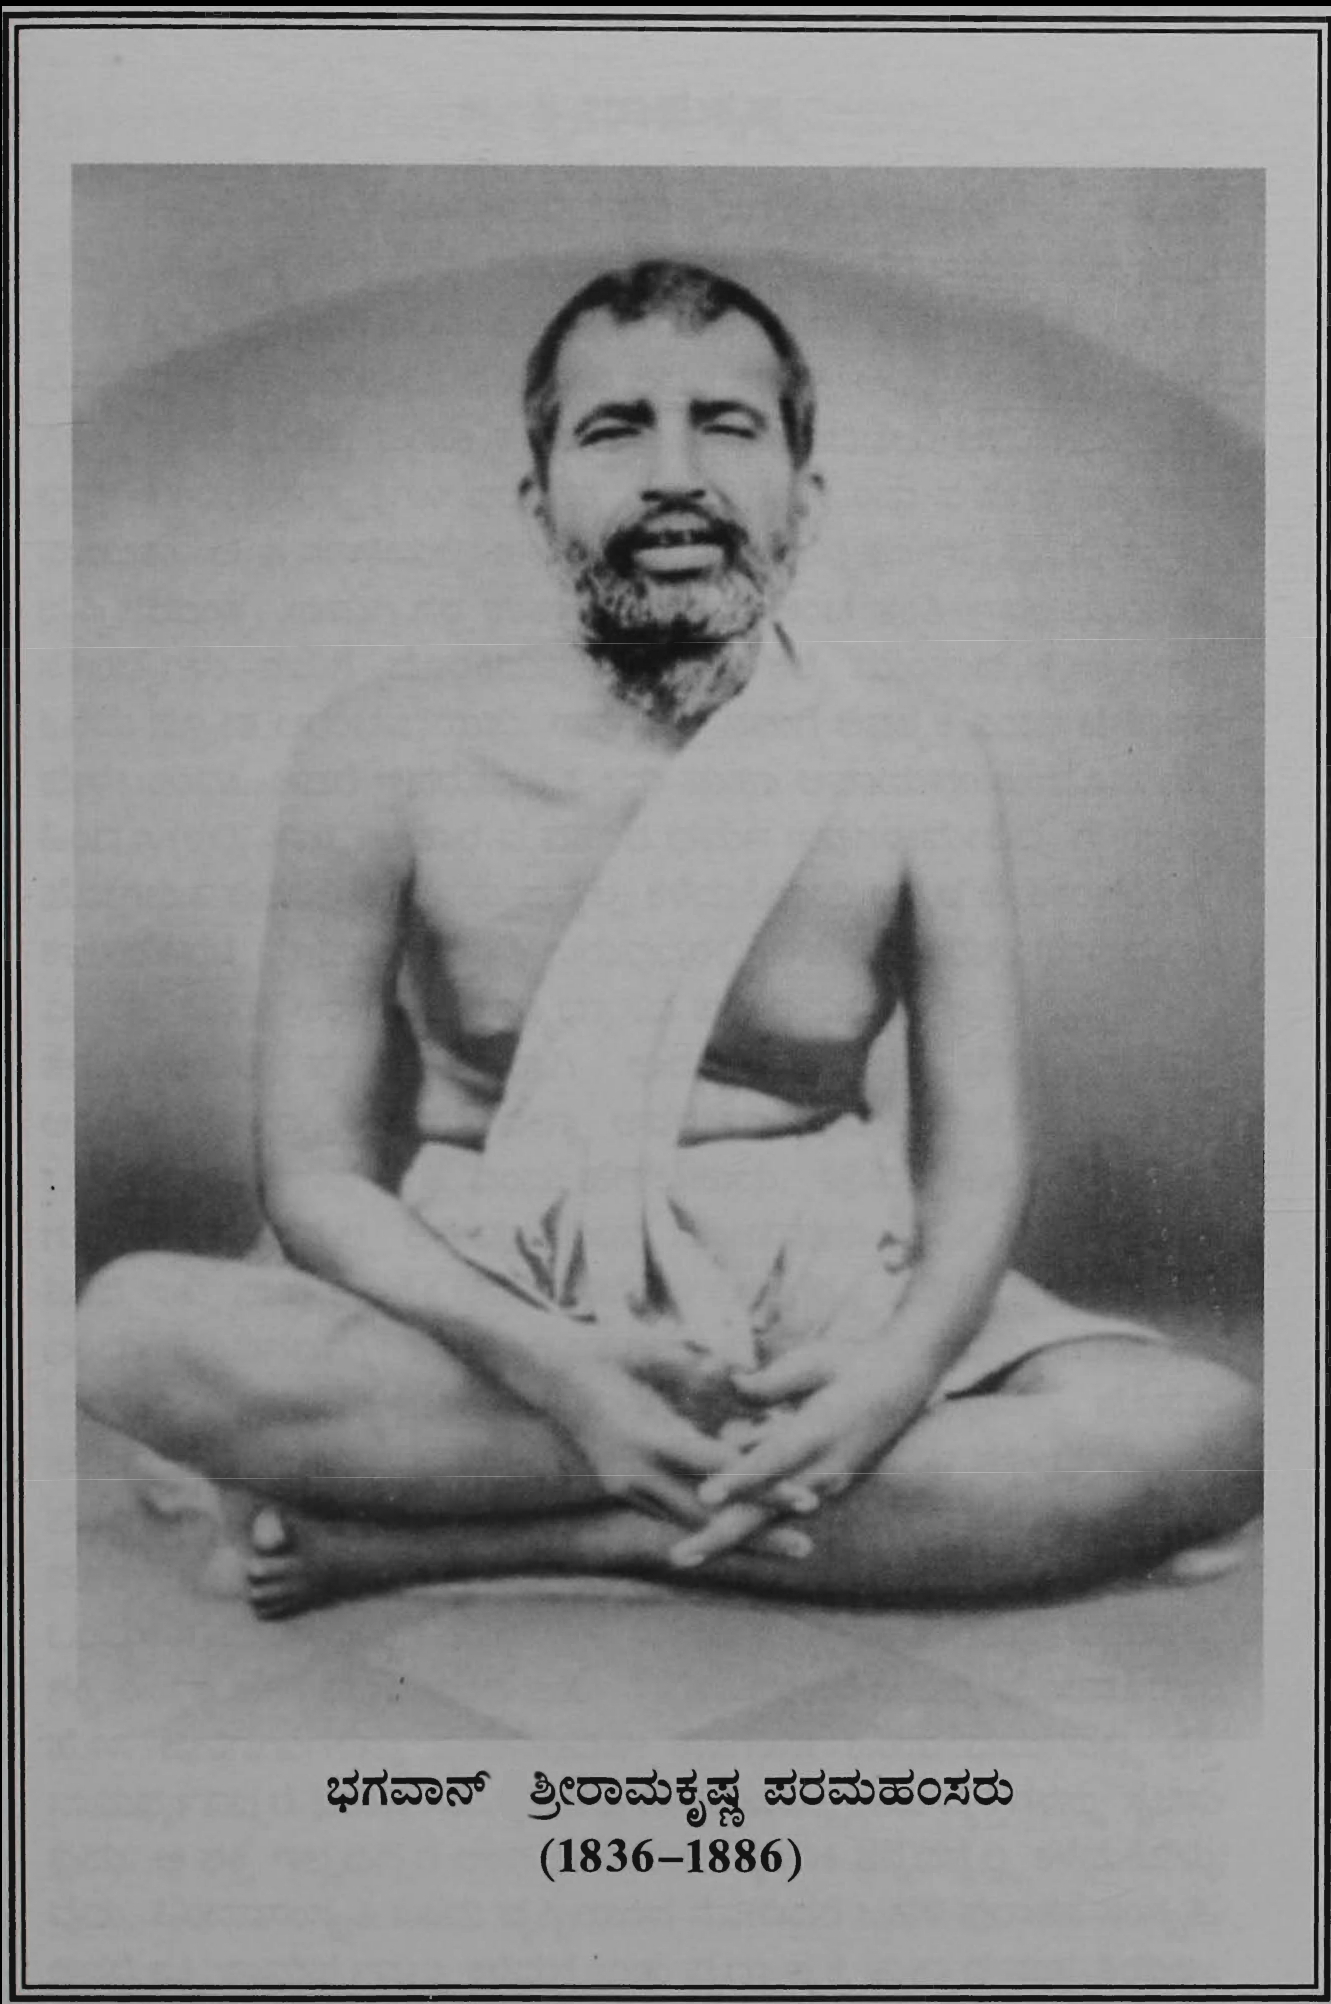
\includegraphics[scale=0.87]{images/1.jpeg}
\end{figure}

